A programmable computer is a gadget without precedent that can be appreciated
from many perspectives. For example, it can be viewed as an engineering marvel
of ever-increasing capacity, as a medium for new flashy applications, or as the
machine-independent scientific discipline that forms its
foundations~\cite{dijkstra1979a,hoare2006}. This dissertation focuses on the
intellectual challenge of \emph{programming} these gadgets.

\begin{quotation}
\noindent This challenge seems unique in the combination of the possibility for
unmastered complexity -- programs are among the most complex things ever
conceived -- and the ultimate, but misleading, simplicity of a world of zeros
and ones alone~\cite{dijkstra1979a}.
\end{quotation}

Programming languages provide us a convenient interface for crafting programs. A
programming language is an {abstraction layer}, because it relieves us from
working with 0s and 1s directly. We can write programs in a human-intelligence
form, and then \enquote{translate} (compile) it to 0s and 1s for processing by
computers. However, the abstraction provided by programming languages does
nothing to reduce the intellectual challenge involved in
programming~\cite{dijkstra1979b}. If we write a syntactically legal but faulty
program, we are at the mercy of our faulty creation when the program executes.

\paragraph*{Equivalence}
A fascinating feature about programs is that we can write multiple distinct
programs that compute the same result for the same input. Two programs
$\sem{p_1}$\symbo{funprog} and $\sem{p_2}$\symbo{funprog} are functionally
\emph{equivalent}\index{functional equivalence}, \ie \(\sem{p_1} \equiv
\sem{p_2}\)\symbo{equiv}, iff for every possible input \(i\), \(\sem{p_1}(i) =
\sem{p_2}(i)\)\symbo{funprog}. In other words, the criteria is to maintain the
input/output behavior, but we are allowed to change \emph{how} the result is
computed. A scientifically inclined reader will recognize \ndx{functional
equivalence} as multiple algorithms computing the same function. A software
engineer will recognize it as the art of \ndx{refactoring}.

To demonstrate the idea, consider the two programs in~\autoref{lst:intro}. The
programs consider two \enquote{input variables}, \pr|X| and \pr|Y|, and store
the result in variable \pr|Z|. The variable \pr|bit| is either \(0\) or \(1\).
By visual inspection, it is obvious that the programs look different. Yet, for
all values of \pr|X| and \pr|Y|, they compute the same result.\footnote{This is
an informal claim, and it will be revisited
in~\autoref{subsubsec:sm-tool-examples}.} The programs are thus functionally
equivalent\index{functional equivalence}.

\begin{center}
\captionsetup{type=lstlisting}
%! suppress = FileNotFound
\begin{minipage}{.3\textwidth}
\lstinputlisting[
      nolol,label={lst:p1},frame=none,numbers=none,
      aboveskip=0pt,belowskip=0pt]{equiv1.imp}
\end{minipage}%
\hspace{5em}%
%! suppress = FileNotFound
\begin{minipage}{.4\textwidth}
\captionsetup{type=lstlisting}
\lstinputlisting[
      nolol,label={lst:p2},frame=none,
      numbers=none,aboveskip=0pt,belowskip=0pt]{equiv2.imp}
\end{minipage}
\captionof{lstlisting}[Equivalent programs]{Equivalent programs.}
\label{lst:intro}
\end{center}

It is natural to ask, \enquote{which program is better?} The program on left
contains no arithmetic operations. Its behavior is easy to read and understand
from how the program is written. The clarity is a useful if the program is
intended for frequent visual inspection. However, we may not care about
readability. Many programs, like the ones generated by a compiler, are never
read by humans. The program on right has the advantages that it does not involve
conditional branching and always evaluates the full arithmetic expression. Such
features are beneficial in certain application domains, like information
security (discussed in~\autoref{pl-sec}). Therefore, choosing the preferable
program form depends on what is meant by \enquote{better}. A question of
interest is how can we quantify and measure such aspects of programs?

\paragraph*{Non-functional properties}
Extending beyond functional behavior, we evaluate programs based on their
quality attributes, \ie \emph{non-functional properties}\index{non-functional
property}. Non-functional properties include aspects like program security and
resource consumption. For example, between two functionally equivalent programs,
we may want to identify the program that computes the result faster or using
less memory. A main theme of this dissertation is to treat \emph{programs as
mathematical objects} to \emph{analyze their non-functional properties}. Among
the goals are developing techniques that enable quantifying such properties.
Furthermore, instead of trusting informal claims---like the earlier one about
program equivalence---we seek rigorous guarantees that the stated properties
truly hold in the inspected program(s).

\paragraph*{Scientific challenges}
The challenge of programming thus involves much more than \enquote{just} the act
of writing functionally correct programs. How to achieve desirable behaviors and
exclude bad ones, and how to detect desirable non-functional properties in
programs are scientifically independent and compelling questions.

\subsection{Dissertation Core Topics}
\label{subsec:dissertation-themes}

The quest to analyze non-functional properties in programs brings us to the
topic of static program analysis. In addition, obtaining strong guarantees
requires formal methods. These are the two core topics of this
dissertation. For a higher sense of adventure, and to make the dissertation
exploration worthy of a multi-year doctoral study, we add \emph{implicit
computational complexity} to the list of topics.

\paragraph*{Static program analysis and formal methods}
The goal in program analysis is to inspect programs and check whether they
satisfy some desirable behavioral criterion. While many families of techniques
exist, this dissertation focuses on analyzing programs statically, \ie by how
programs are written. Static analysis techniques study program syntax. They aim
to make judgements about how the program will behave when it is executed, but
without ever executing the program. Formal methods complement the setting by
providing the mathematical techniques and tools to obtain rigorous guarantees.
Formal methods enable providing \emph{proofs} about the conclusions of
(informal) program analysis. This way, we can substitute informal claims with
maximally strong assertions.

\paragraph*{Implicit computational complexity}
The core idea of implicit computational complexity (ICC) is to quantify
computational power through programming languages. Although ICC can be viewed
from many perspectives, in the scope of this dissertation, its role is to
provide a conceptual \enquote{toolbox} for constructing techniques of static
program analysis. Considered broadly, ICC finds ways to characterize program
properties---mainly resource consumption---by introducing a restriction at the
level of a programming language. The restriction is such that it guarantees the
target property holds in every expressible program. Programming languages thus
become a \emph{mechanism} to guarantee ideal runtime behavior. There are
multiple compelling motivations for this approach. For example, ICC drives
better understanding of resource consumption and provides natural ways to
express and control resources usage of programs~\cite{kristiansen2017}. Because
behavioral guarantees are part of the language design, this creates a
\emph{temporal shift} that enables reasoning about properties \emph{before} any
program exists. If we can identify the construction principles of satisfactory
programs, this would remove the need to analyze programs after they are written.
However, materializing such ideas in practice requires deeper investigations of
implicit computational complexity.

\begin{infobox}[]{Primary topics summarized}
The dissertation investigates problems in {static program analysis}, ideally
with {formally verifiable guarantees}, and from the starting point of {implicit
computational complexity}.
\end{infobox}

\subsection{Addressed Problem}
\label{subsec:problem}

Given the many compelling motivations, there exists a long series of theoretical
results in implicit computational complexity (reviewed
in~\autoref{icc-theories}). These works focus primarily on \emph{defining}
theoretical systems. There are substantially fewer explorations of
\emph{applications} of those theories (see~\autoref{resource-analysis-tools}
and~\autoref{icc-sec} for related presentations).\footnote{By
\enquote{application}, we refer to any use case beyond \ndx{complexity theory},
including implementations.} The difference in allocated efforts could be
explained by many factors, including the following.\footnote{The claims come
from observations and conversations; they are unlikely to exist in literature.}

\begin{enumerate}

\item \emph{Broad insight is required to identify suitable application domains.}
      The claim is evidenced by, \eg \ndx{Parikh's Theorem} from \ndx{automata
      theory}. Classically, the theorem is about letter-counting and language
      \ndx{expressiveness}. Its practical usefulness was enabled only
      \emph{decades later} by the development of efficient algorithms. Since
      then, it has been exploited in a range of applications like SMT solvers,
      verification of cryptographic\index{cryptography} protocols and
      \ndx{concurrent programs}, and query evaluations in \ndx{graph
      database}s~\cite[pg. 2]{hague2024}.

\item \emph{There is a conceptual gap between pure theory and practical
      applications.}
      For example, the flow calculus of mwp-bounds (reviewed
      in~\autoref{flow-calculus}) was designed for theoretical analysis of
      programs. Although the initial presentation~\cite{jones2009} seems to
      provide an automatable technique, much subsequent work was needed to
      materialize this objective. In general, it is extremely difficult to
      foresee application challenges without attempting to bridge the gap.

\item \emph{An application may require changing the research domain.}
      For example, a result in theoretical computer science may find relevant
      uses in \ndx{formal verification}, \ndx{symbolic execution}, or
      \ndx{secure compilation}. The cross-domain adaptation then requires
      communicating findings to new communities who may be motivated differently
      to assess the usefulness of the findings.

\end{enumerate}

Some application challenges are specific to implicit computational complexity.
Restricting a programming language sacrifices \ndx{Turing-completeness}. A
non-Turing-complete programming language means certain programs become
inexpressible. The task of writing (or finding) a satisfactory program is then
delegated upstream to the software engineer~\cite[p. 14]{moyen2017}. If the
restriction is too strong, it is difficult, or perhaps impossible, to express
natural algorithms. This creates a trade-off between theoretical soundness (\ie
providing a guarantee) and \ndx{expressiveness}~\cite{feree2018}. It is thus
justifiable to ask, what are the uses of such restricted programming
languages?\footnote{For an inspirational warm-up, see
\url{https://stackoverflow.com/questions/315340}; a discussion about
practicality of non-Turing-complete languages.\index{Turing-completeness}}

With these considerations in mind, the \emph{main hypothesis} of this
dissertation pushes to investigate the application potential of implicit
computational complexity.

\begin{infobox}[]{Main hypothesis}
Implicit computational complexity offers applied utilities when lifted from the
theoretical domain.
\end{infobox}

\noindent
Every manuscript in this dissertation is an instantiation of this main
hypothesis. Through applications, we can stress test capabilities of ICC
systems; pinpoint limitations and discover use cases in other domains.

\subsection{Dissertation Goals}\label{subsec:specific-aims}

In support of the main hypothesis, we define four actionable goals.

\begin{itemize}[label=\iconBOX]

\item\textbf{Goal 1.}
\emph{Extend applied capabilities in automatic program analysis and
verification.}
The motivation is to show that ICC theories can provide new complementary
techniques for automatic program analysis and support verification of
non-functional properties.

\item\textbf{Goal 2.}
\emph{Take ICC techniques closer to integration with real-world software
development workflows.}
Such integration would drive theoretical improvement, support relevance of ICC
techniques, and motivate thinking about ICC from fresh perspectives.

\item\textbf{Goal 3.}
\emph{Initiate conversations about the relevance of ICC applications.}
Improvements in ICC are typically achieved by showing improvement in
\ndx{expressiveness}. A common strategy is to show that the newly presented
system gives a guarantee for some subset of programs that were not expressible
previously.\footnote{The strategy is used \eg in~\cite[p.16--17]{hainry2023},
~\cite[p. 17]{jones2009}, and~\cite[p. 147]{feree2018}.} However, this strategy
is limited in quantifying practical usefulness of the ICC systems. Particularly,
it does not account for the \enquote{methodological cost} at which the
improvement is achieved. Applications would provide complementary insight and
metrics to assess the capabilities of ICC systems.

\item\textbf{Goal 4.}
\emph{Expose ideas from implicit computational complexity to broader research
communities.}
Wider dissemination of ideas could lead to discovery of new applications and
ease communication about ICC results.

\end{itemize}

The completion of these goals is discussed in~\autoref{sec:res-summary}.

\subsection{Research Plan}
\label{subsec:conn-papers}

To make the main hypothesis and goals more concrete, we define two research
directions. One focuses on \ndx{automatic resource analysis}. The other
investigates the uses of implicit computational complexity in ensuring
non-functional properties (besides complexity). These directions are visualized
in~\autoref{fig:conn_papers}. An alternative way to think about these directions
is that the first aims to apply ICC systems in the originally designed ways,
while the second seeks to discover unexpected applications.

\begin{figure}[p]
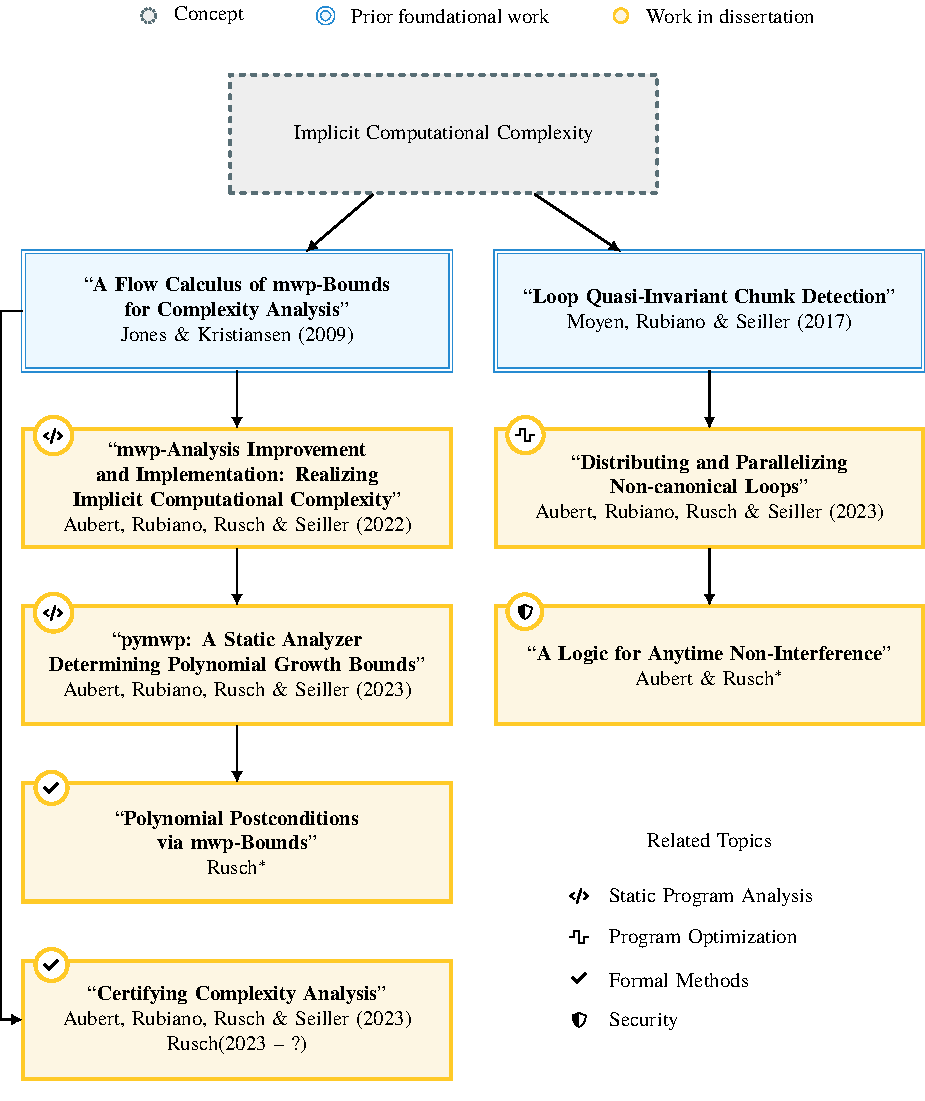
\includegraphics[width=\linewidth,keepaspectratio]
{fig_conn_papers}\vspace{1.5em}
\caption[Dissertation manuscripts and their associations]
{Dissertation manuscripts and their dependency associations.}
\label{fig:conn_papers}
\end{figure}

\subsubsection{Automatic Resource Analysis}
\label{ssec:mwp-rqs}
\index{mwp-calculus}\index{automatic resource analysis}

In the first direction, we focus on the flow calculus of
mwp-bounds\index{mwp-calculus}, introduced by~\textcite{jones2009}. It is a
canonical example of an ICC system for analyzing variable value growth (data
size) in \ndx{imperative programs}. The flow calculus is introduced in detail
in~\autoref{flow-calculus}.

Building on the flow calculus, we define three research questions.
\begin{description}

\item[RQ1] Can we develop an automatic program analysis based on the flow
calculus?

\item[RQ2] Given its paper proofs, is the theory correct? \Ie can we prove
formally the soundness of the flow calculus?\index{soundness of mwp-calculus}

\item[RQ3] Assuming the theory can be automated, what are its use cases?

\end{description}

The manuscripts building on the flow calculus demonstrate its uses in static
program analysis and in formal verification for specification inference. The
manuscripts support all dissertation goals. The manuscripts concerned with the
implementation of the flow calculus (RQ1) support Goals 1--3. A formally
verified soundness proof (RQ2), and an application to formal verification (RQ3)
support Goal 4.

One manuscript, \emph{\enquote{mwp-Analysis Improvement and Implementation:
Realizing Implicit Computational Complexity}} is in the Appendix
(\autoref{app:additional-manuscripts}) due to an Augusta University policy. The
placement should not distract from the significance of the work, as several
other manuscripts follow from it.

Results of the research questions are discussed
in~\autoref{subsec:res-flow-calc}.

\subsubsection{Analyzing Extended Non-Functional Properties}

The second direction starts with complexity-theoretic techniques, but then
repurposes them toward other non-functional properties. The technical foundation
is inspired by \enquote{\emph{Loop Quasi-Invariant Chunk Detection}},
by~\textcite{moyen20172}. In the original formulation, the idea is to identify
fragments of loops (called \enquote{blocks}), whose variables become invariant
after a finite number of iterations. Such loop \ndx{quasi-invariant} code blocks
can then be lifted from the loop. The program transformation improves the loop's
complexity profile if the lifted block is a \ndx{nested loop}. For convenience,
we refer to this technique as the \emph{QI framework}, after
\ndx{quasi-invariant}s.

This original QI framework is not presented in this dissertation. This is
because each refinement changes the behavior of the system and requires fully
redefining the system each time. The manuscripts in~\autoref{sec:vmcai}
and~\autoref{sec:anytime} thus provide the technical details.

We define two research questions relating to the QI framework.

\begin{description}

\item[RQ4] How to develop a program transformation to increase parallelization
potential?

\item[RQ5] How to use it to analyze security properties, specifically
non-interference?

\end{description}

The research questions thus change the motivation from \ndx{complexity theory}
to other application domains. Critically, the original complexity result may be
lost, but some other guarantee is gained. On the surface, the research questions
appear to be about properties, but more deeply they are about understanding
better the underlying theory and its flexibility.

Both goals are practically motivated. The expected deliverables support Goals
1 and 2. Moreover, they are strongly aligned to support Goal 4.

The results of the research questions are discussed in~\autoref{subsec:res-qi}.

\subsection{Manuscript Overview}
\label{ssec:manuscripts}

The dissertation manuscripts connect implicit computational complexity with
related research topics. Each manuscript is decorated with an icon that denotes
the secondary topic. The topics include static program analysis \iconSPA,
security \iconSEC, program optimization \iconOPT, and formal methods \iconFM.


\paragraph*{Author contributions}
The authors are always listed in alphabetical order. The manuscripts in
Chapters~\autoref{published-manuscripts}--\autoref{ch:unpublished-research} are
\enquote{first author} works. The manuscripts in
Chapter~\autoref{app:additional-manuscripts} are \enquote{non-first author}
works. The co-authors contributions are detailed in
Chapter~\autoref{app:sec:coauth}.

\paragraph*{Peer review}
The entire Chapters~\autoref{published-manuscripts},
~\autoref{ch:unpublished-research}, ~\autoref{ch:summary},
and~\autoref{app:additional-manuscripts} have been peer reviewed. In other
words, the only new content is Chapters~\autoref{introduction}
and~\autoref{ch:discussion}, \ie Introduction and Discussion.

\begin{itemize}

\item The published works in Chapters~\autoref{published-manuscripts}
and~\autoref{app:additional-manuscripts}, were inspected by 7--10 reviewers
before acceptance.

\item The unpublished works, in Chapter~\autoref{ch:unpublished-research}, have
been reviewed by at least 4 reviewers thus far. Preliminary versions have been
accepted and presented at respectable workshops. Be advised that the unpublished
works must be viewed with caution, as they are works in progress. All works have
some limitations that prevent their inclusion among the published manuscripts.

\item Chapter~\autoref{ch:summary} is an extended abstract. It describes about
the full-length dissertation in a standalone manner. It has been peer-reviewed
and presented at the
\href{https://2025.ecoop.org/track/ecoop-2025-doctoral-symposium}{Doctoral
Symposium} of \href{https://2025.ecoop.org}{the European Conference on
Object-Oriented Programming}.

\end{itemize}

\subsection{Important Tips to the Reader}
\label{subsec:tips}

This dissertation contains three varying-length versions of its content.
This allows accessing the presentation at different levels of detail, by need.

\begin{infobox}[]{Content organization}
\begin{enumerate}[wide, labelwidth=!, labelindent=0pt]

\item The \emph{\hyperref[abs]{abstract}} contains the highlights only.

\item \emph{Chapters~\autoref{introduction}--\autoref{ch:discussion}
and~\autoref{app:additional-manuscripts}} form the full-length presentation.

\item \emph{Chapter~\autoref{ch:summary}} is a standalone extended summary of
the full presentation.
\end{enumerate}
\end{infobox}

\subsubsection{Software Artifacts and Data Availability}

All software developed as part of this dissertation is publicly available. Each
published manuscript in the dissertation has an associated software artifact.
The artifacts are archived, according to the policies of the Association for
Computing Machinery~\cite{acm_badging}, for long-term retention. The artifacts
are archived even if the publication venue did not provide an official artifact
evaluation round. Therefore, each manuscript consists of more than just the text
pages of the dissertation. How to locate the artifacts is explained
in Chapter~\autoref{app:sec:artifacts}.


\paragraph*{Dissertation source code}
The source code of the dissertation~\cite{diss} is publicly available at the
following repository.

\noindent\begin{minipage}{\textwidth}
%! suppress = EscapeUnderscore
\begin{browserlisting}[nolol,escapeinside=!!]
!\href{https://github.com/nkrusch/dissertation}
{\texttt{https://github.com/nkrusch/dissertation}}!
\end{browserlisting}
\end{minipage}

\paragraph*{Artifact}
The dissertation has a companion artifact. It is preloaded with all required
software and it enables reproducing the executable examples that appear in the
dissertation. For example,~\autoref{sec:toolguide} can be followed interactively
with the artifact. The artifact URL is

\noindent\begin{minipage}{\textwidth}
%! suppress = EscapeUnderscore
\begin{browserlisting}[nolol,escapeinside=!!]
!\href{https://doi.org/10.5281/zenodo.15288399}
{\texttt{https://doi.org/10.5281/zenodo.15288399}}!
\end{browserlisting}
\end{minipage}

\subsubsection{Notational Conventions}

\paragraph*{Programming languages, syntax, and code blocks}
Syntactic constructs (variables, expressions, commands, \etc) that are embedded
in text are typeset in \pr|teletype|. Larger or more significant code blocks are
displayed as dedicated code listings. The listings will display, in the bottom
right corner, the associated programming language or context, according
to~\autoref{tab:pls}. In the table, \emph{version} is the language release
version assumed in the listings, when applicable (pseudo-languages do not have a
version). Plain text listings, that describe command outputs, are labelled
\enquote{output.} Internet addresses are marked by \langclr{cweb} \enquote{www.}
The \ndx{Rocq} Prover is undergoing a name change from its former name
Coq\index{Coq|seealso{Rocq}}. We will use the new name whenever possible.

\begin{table}[h]
\begin{center}
\begin{tabular}{@{}lllc@{}}
\toprule
\multicolumn{2}{@{}l}
{\textbf{Language}} &
\textbf{Description} &
\textbf{Version} \\
\midrule
\langclr{cc}        & C           & the \ndx{C} programming language & C99 \\
\langclr{ccstar}    & C*          & imperative C-like pseudo-language & -- \\
\langclr{cces}      & CES         & \ndx{cost equation system} &  -- \\
\langclr{ccmd}      & cmd         & executable shell/terminal command & --  \\
\langclr{cdafny}    & Dafny       & the \ndx{Dafny} programming language & 4.10.0 \\
\langclr{cimp}      & Imp         & imperative language of \ndx{mwp-calculus} & -- \\
\langclr{cjava}     & Java        & the \ndx{Java} programming language & SE 24 \\
\langclr{compcode}  & OMP         & C code that includes \ndx{OpenMP} directives & 6.0 \\
\langclr{crocq}     & Rocq        & the \ndx{Rocq} interactive theorem prover & 8.20.1 \\
\langclr{cmathc}    & SSReflect   & the \ndx{SSReflect} proof language & 2.4.0 \\
\langclr{cwhile}    & While       & simple imperative while language & -- \\
\bottomrule
\end{tabular}\end{center}
\caption[The programming languages of code listings]
{The programming languages used in code listings.}
\label{tab:pls}
\end{table}

\paragraph*{Line numbers}
References to a line of source code (or an algorithm) begin with an L, for
\underline{l}ine. The L is followed by a number (or a numeric range) that
specifies the row(s) of interest. For example, L3 means \emph{line number 3},
and L10--12 means \emph{lines 10 to 12}.

\paragraph*{Distinguishing variable states}
We will often want to refer to the same variable in different states of
computation. In the style of \emph{\ndx{Z specification
language}}~\cite{spivey1992}, we use notation that identifies the \emph{new}
(post) states. A plain variable refers to a state where the variable holds its
{initial} value. A variable with a postfix decoration \pr|'| refers to a state
where the variable holds its {final} value. For example, \pr|X| refers to the
initial value and \pr|X'| refers to the final value.

\subsubsection{Lookup Indices}

The dissertation includes three indices for terms, acronyms, and symbols. The
Term Index (\autoref{sec:app:index}) lists technical terms and their uses.
Acronyms are generally defined at first use and the Index of Acronyms
(\autoref{glo:acr}) lists the long form. The Symbol Index (\autoref{glo:symb})
lists definitions of symbolic notations.

\subsubsection{Dynamic Bibliographic Entries}
\label{sssec:dyn-bib}

Some bibliography entries refer to dynamic resources like software, web pages,
or lecture notes (without DOIs). References to such documents may become
unreliable over time. To improve the long-term availability and recoverability,
they are pre-emptively preserved in suitable online archives, on \ndx{Software
Heritage} and the \ndx{Internet Archive}.

\paragraph*{Software repositories}
Version-controlled third-party software repositories are archived at
\href{https://softwareheritage.org}{\ndx{Software Heritage}}. For a repository
hosted at \pr|<URL>|, the recovery address pattern is:

\noindent\begin{minipage}{\textwidth}
%! suppress = EscapeUnderscore
\begin{browserlisting}
!\texttt{https://archive.softwareheritage.org/browse/origin/directory/}!
!\hspace{2em}\texttt{?origin\_url=<URL>}!
\end{browserlisting}
\end{minipage}

\begin{example}[Recovering a software repository]
The dissertation source code archival recovery address is:\mbox{}

\noindent\begin{minipage}{\textwidth}
%! suppress = EscapeUnderscore
\begin{browserlisting}
!\texttt{\href{https://archive.softwareheritage.org/browse/origin/directory/?origin_url=https://github.com/nkrusch/dissertation}{https://archive.softwareheritage.org/browse/origin/directory/}}!
!\hspace{2em}\texttt{\href{https://archive.softwareheritage.org/browse/origin/directory/?origin_url=https://github.com/nkrusch/dissertation}{?origin\_url=https://github.com/nkrusch/dissertation}}!
\end{browserlisting}
\end{minipage}
\end{example}

\paragraph*{Written documents}
Web pages and PDF files are archived in the \ndx{Wayback Machine} of the
\ndx{Internet Archive}. Use the following pattern to recover a document from the
Internet Archive -- substitute \pr|<URL>| by the document's URL\@:

\noindent\begin{minipage}{\textwidth}
%! suppress = EscapeUnderscore
\begin{browserlisting}
!\texttt{https://web.archive.org/web/<URL>}!
\end{browserlisting}
\end{minipage}

A few cited documents could not be archived by the Internet Archive; for example
because the hosting server was blocking automatic clients. There is a copy of
these documents is in the dissertation companion artifact~\cite{aicc}.

\begin{example}[Recovering archived documents]

The following URL is fragile and it may disappear in the future.\mbox{}

\noindent\begin{minipage}{\textwidth}
%! suppress = EscapeUnderscore
\begin{browserlisting}
!\texttt{\url{https://types22.inria.fr/files/2022/06/TYPES_2022_paper_14.pdf}}!
\end{browserlisting}
\end{minipage}

As a backup, the following Internet Archive address produces the same
document.\mbox{}

\noindent\begin{minipage}{\textwidth}
%! suppress = EscapeUnderscore
\begin{browserlisting}
!\texttt{\href{https://web.archive.org/web/https://types22.inria.fr/files/2022/06/}{https://web.archive.org/web/https://types22.inria.fr/files/2022/06/}}!
!\hspace{2em}\texttt{\href{https://web.archive.org/web/https://types22.inria.fr/files/2022/06/TYPES_2022_paper_14.pdf}{TYPES\_2022\_paper\_14.pdf}}!
\end{browserlisting}
\end{minipage}
\end{example}
